\section{Lucinde}%
\label{sec:Lucinde}
\begin{quotex}
Update 12 October 2021. Thus began the path of the Knight 15 years ago, today.

\end{quotex}
From Lucinde by \textbf{Friedrich Schlegel}.

\textbf{Julius writes to Lucinde:}

\begin{quotex}
In the holy solitude around me everything was light and color, and a fresh warm breath of life and love touched me, and stirred and murmured in all the branches of the luxuriant grove. I looked, and I delighted in everything at the same time: the vigorous green, the white blossom, and the golden fruit. And so too with the eye of my spirit I saw the one and only and forever beloved in many forms: sometimes as a childlike girl, sometimes as a woman in the full bloom and strength of love and femininity, and sometimes as a worthy mother with her earnest little boy in her arms. I breathed the spring, saw clearly the eternal youthfulness around me, and I said with a smile: “Even if this world is not the best or the most useful, still I know that it is the most beautiful.”

Nothing could have shaken me in this feeling or conviction, neither general doubt nor my own fear. For I believed I was looking deeply into the secrets of nature; I felt that everything lived eternally and that even death was only an amiable deception. But, actually, I didn't think about it very much — at least I wasn't particularly disposed to classify and analyze abstract concepts.

Instead I lost myself gladly and deeply in all the comminglings and intertwinings of joy and pain from which come the savor of life and the bloom of feeling, spiritual voluptuousness as well as sensual beatitude. A subtle fire flowed in my veins; what I dreamed of wasn't just a kiss or the embrace of your arms; it wasn't just a wish to break the tormenting thorn of yearning and cool the sweet flames in surrender; I didn't yearn only for your lips or your eyes or your body.

It was, rather, a romantic confusion of all these things, a wonderful mixture of the most various memories and yearnings. All the mysteries of male and female frivolity seemed to hover about me as suddenly your real presence and the gleam of blooming happiness on your face inflamed my lonely self. Wit and rapture alternated between us and became the common pulse of our united life and we embraced each other with as much wantonness as religion.

I begged you that for once you might give yourself completely over to frenzy, and I implored you to be insatiable. Still, I listened with cool composure for every faint sign of bliss, so that not a single trace might escape me and leave a gap in our harmony. I didn't simply enjoy, but felt and enjoyed the enjoyment itself.

\end{quotex}
It may seem presumptuous to include love advice in a discussion on \emph{jnanis}, since we associate them with asceticism and celibacy. However, while it started somewhat “tongue-in-cheek”, there is a valid purpose. If non-duality is true, then every area and aspect of life is non-dual. We cannot see the ascetic as the norm — it's odd that only now are we concerned about the termination of human life on earth, whether through war or environmental destruction, when in actuality, it has always been the human prerogative to end the world simply by refusing to reproduce!

It is a sign of the times to believe we have evolved to the point of accepting practices which have traditionally been considered deviant, on the grounds that they are “natural”. However, this assumes a profound misunderstanding of man, who is anything but natural, both in a positive and a negative sense. Positively, man is more than his nature; with his source in Atman, he creates himself and cannot be reduced to biology, instinct, and impulse. To the modern mind, freedom means release from every constraint to say “yes” to every whim. However, the task of self-creation will often require a “no” instead. It will serve no point to be more specific; as in everything, prudence and wisdom will be suitable guides. Keep in mind, though, the Hermetic principle: “As above, so below”. The manifest world arises from the polarity of the male and female principles (\emph{Purusha} and \emph{Prakriti}). The most creative relationships will exhibit that polarity in the phenomenal realm.

Negatively, man does not understand his true nature. As we pointed out, his perceptions, actions, and thoughts are delusory, so man, in this unregenerate state, cannot even know his true nature, so what he considers “natural” is, from a metaphysical perspective, more likely to be the manifestation of unnatural \emph{tamasic} forces. Keep in mind that the studied “naturalness” of a Zen practitioner, or the “naturalness” of a dancer or artist, are actually the result of deep and dedicated practice.

In the past, we have quoted from \textbf{Friedrich Schlegel}`s novel \emph{Lucinde} without giving the background. Schlegel was a founder of the Romantic movement in XIXth century German art and was an innovator in bringing the Vedic teachings to Europe. The common “wisdom” among the intelligentsia at that time, was that a man needed three types of women to be fulfilled: a wife, a mistress, and an âme-soeur (soul sister). The first two are self-explanatory. But the âme-soeur is a Platonic relationship; she is able to discuss the deep things of life (e.g., art, philosophy, spirituality, etc.).

\begin{wrapfigure}{rt}{.4\textwidth}
\centering
 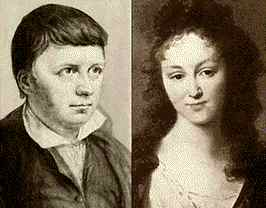
\includegraphics[scale=.5]{a20061012Lucinde-img001.jpg} 
 \caption{Friedrich and Dorothy Schlegel}
\end{wrapfigure}

Schlegel and his wife, Dorothy, turned that common wisdom on its head by incorporating all three aspects into a single relationship. The progress and results of that experiment were documented in his novel.

While the “mate” (or wife) can be seen as the public face of the relationship, the Mistress is the private face. (This is why any hint of promiscuity, adultery, exhibitionism betrays the relationship.) The public/private distinction corresponds to the exoteric/esoteric distinction in religions. So, exoterically, since sexual relations between mates is open to biological life, by correspondence, esoterically, the Mistress relationship is also open to the creation of a new life, though, in this case, it is the spiritual birth of a new being, wherein they each find their own wholeness in the other. So for Schlegel, the âme-soeur relation is not opposed to a “conventional” relationship, but is instead its fulfillment.

This extended passage from Lucinde is illustrative:

\begin{quotex}
Yes: I would have thought it a fairy tale that there could be such happiness and such love as I feel now — and such a woman, at once the most delicate lover, the most wonderful companion, and the most perfect friend. For in friendship particularly I sought for all that I lacked and didn't expect to find in any woman. In you I've found everything and even more than I could have hoped for; but, then, you're not like the others. You're untouched by the faults that custom and caprice call female. Aside from your little idiosyncrasies, the femininity of your soul consists simply in your making life and love synonymous. You feel completely and infinitely; you know of no separations; your being is one and indivisible. That is why you are so serious and so joyful. That is why you take everything so solemnly and so negligently, and also why you love me completely and don't relinquish any part of me to the state, to posterity, or to my friends.

Everything belongs to you, and we are in every respect closest to each other and understand each other best. You're at my side at every stage of human experience, from the most passionate sensuality to the most spiritual spirituality; and only in you have I seen true pride and true womanly modesty.The most extreme sorrows, if they merely enveloped us and didn't separate us, would seem to me nothing more than a refreshing contrast to the sublime frivolity of our marriage. Why shouldn't we interpret the bitterest whim of chance as a lovely witticism and an exuberant caprice, since we, like love, are immortal? I can no longer say my love or your love: both are identical and perfectly united, as much love on one side as on the other, This is marriage, the timeless union and conjunction of our spirits, not simply for what we call this world or the world beyond death, but for the one, true, indivisible, nameless, unending world, for our whole eternal life and being.
\end{quotex}
\flrightit{Posted on 2006-10-12 by Cologero }

\begin{center}* * *\end{center}

\begin{footnotesize}\begin{sffamily}



\texttt{Tannheuser on 2021-02-15 at 13:50 said: }

It may be worth meditating on whether there is a parallel between the Mother/Mistress/Ame-soeur triad and the Three Marys (John 19:25) from the New Testament. The fact that all of these important women in the New Testament are named “Mary” would seem to indicate that they are in a some sense different aspects of the same personage.

Magdalene is described as being cleansed of seven devils (Luke 8:2), and the first to behold the resurrected Christ (John 20:11-18). She is also prominent in the apocryphal and “gnostic” gospels — in the Gospel of Mary she describes exclusive and private revelations given to her by Christ, regarding the nature of the soul and spirit, and the trials the soul undergoes after death.

In all of this it's hard not think of Arcanum II of the Tarot, the High Priestess. Tomberg says that she embodies Gnosis, and if we think of Magdalene this way it makes sense that Aquinas calls her “Apostle to the Apostles”:

“Note the three privileges given to Mary Magdalene. First, she had the privilege of being a prophet because she was worthy enough to see the angels, for a prophet is an intermediary between angels and the people. Second, she had the dignity or rank of an angel insofar as she looked upon Christ, on whom the angels desire to look. Third, she had the office of an apostle; indeed, she was an apostle to the apostles insofar as it was her task to announce our Lord's resurrection to the disciples. Thus, just as it was a woman who was the first to announce the words of death, so it was a woman who would be the first to announce the words of life.” (2519)


\hfill

\texttt{Sibylle on 2023-06-05 at 03:16 said: }

Lucinde writes to Julius:

“…childlike cheerfulness and bitter pain, untamed rage and pouring dreams, death and love, desire and contemplation, sweeping exuberance and melancholy, (sweet little sighs of which none escaped my ears), dark sorrow and bright willfulness; this is what I see before me in such clear and powerful manner, gazing at me, living and striving in … letters and dreams, conversations and speeches; this is the spirit and intent of your opus, and that is why it is so dear to me, why I have taken it into my heart, out of intimate love and deep awe; it is here where I have found the clearest image of my own highest longing.”

— Fragment from the appendix of “Lucinde, Studienausgabe”, Reclam Verlag


\end{sffamily}\end{footnotesize}
